\section{Active learning (stage 1)}
\label{sec:visualizer:al}

The main goal of stage 1 is to learn the user's interests. This requires the 
system to select (``query'') data for the user (the ``oracle'') to label 
(``classify''). The VS data for the active learning component is composed of 
all observations of characteristic features (as described in 
Section~\ref{sec:visualizer:scatterplot:features}) for all $n\choose2$ pairwise 
scatter plots of the \textit{actual} data set. This is \textbf{stage 1}. 
The learner may then utilize 
a classification model (discriminant analysis, naive Bayes, decision tree(s), 
logistic regression, etc.) that trains on the labeled data to ``learn'' user 
interests. The user's interests are encoded in a final classifier (some 
instance of 
the classification model) that is applied to automatically label the rest of 
the data. Here again, it is important to be careful about the terminology 
usage. For more on the semantic differences between ``classification model'' 
and ``classifier'' in this thesis, see 
Figure~\ref{fig:visualizer:al:tree}. This is 
\textbf{stage 2} (Section~\ref{sec:visualizer:plotgeneration}). 
It is important to make the stage 1 process as efficient as possible to avoid 
redundancy for the end user. There are various methods that may be used for 
querying in stage 1 as described by Dasgupta~\cite{dasgupta2011}:

\tablespacing
\begin{itemize}
	\item \textbf{Supervised learner}: This learner queries a random 
	subset of all unlabeled data. It ignores the rest of the data when refining 
	the classifier.
	\item \textbf{Semisupervised learner}: Similar to a supervised learner, a 
	semisupervised learner queries a single, random subset of all 
	unlabeled data but proceeds to utilize the remaining unlabeled data to 
	better inform the final classifier.
	\item \textbf{Active learner}: An active learner selects its queries in a 
	non-random, intelligent manner.
\end{itemize}
\bodyspacing

It has been 
shown that when a learning algorithm is allowed to choose its next query, it 
performs better with less training; as such, we choose to utilize active 
learning to select the scatter plots to be queried by the oracle in stage 
1~\cite{settles2010}. This section is primarily focused on the active learner's 
role in the overall system; Chapter~\ref{ch:al} goes into detail on different 
active learning methodologies.

\begin{figure}[htb]
	\begin{center}
		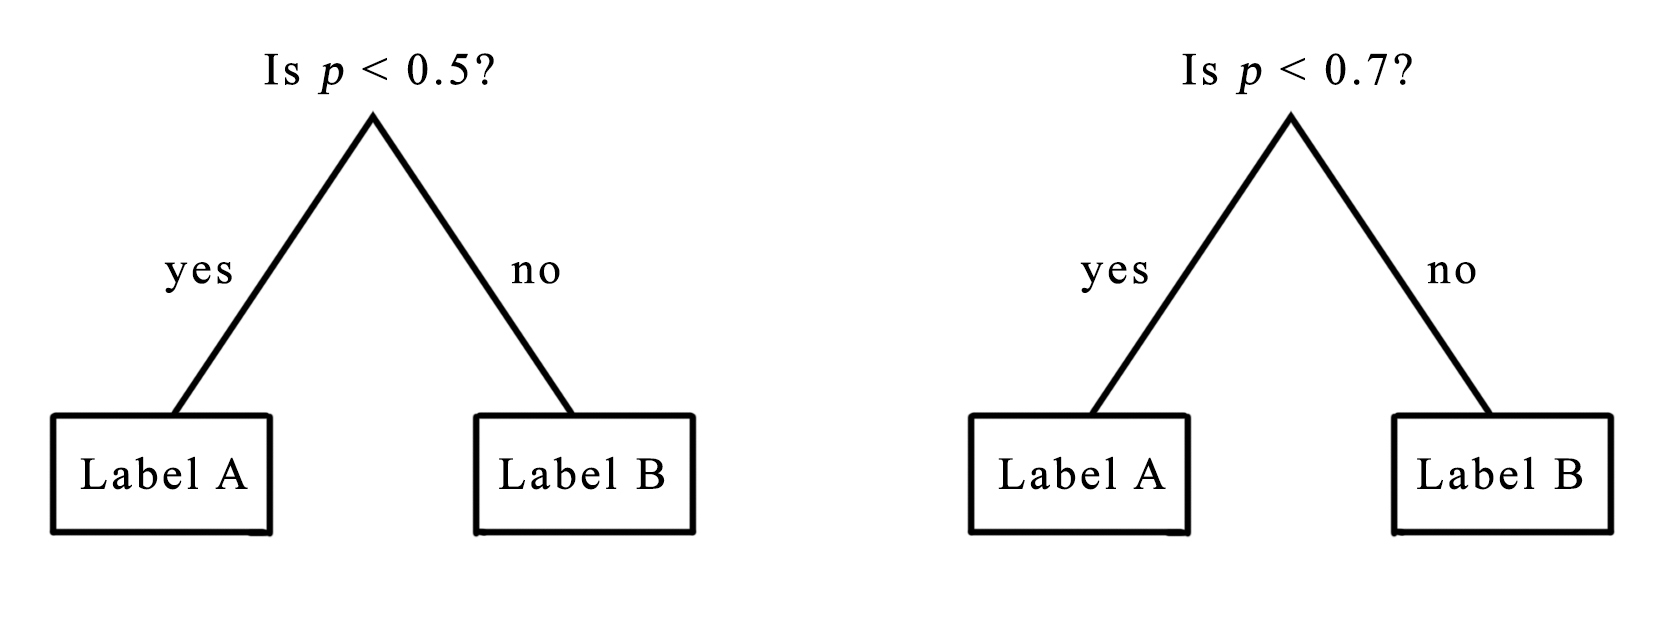
\includegraphics[width=0.75\linewidth]{ch-visualizer/figures/tree}
		\caption[Classifiers and classification models]{Although both figures 
		on the left and right are slightly different classifiers, they 
		are both instances of (extremely simple) decision trees, a type of 
		classification model. Other models include discriminant analysis, naive 
		Bayes, random forest, logistic regression, etc. 
		See Section~\ref{sec:visualizer:plotgeneration:tree} for more details 
		on trees.}
		\label{fig:visualizer:al:tree}
	\end{center}
\end{figure}

\subsection{Initialization of active learner}
\label{sec:visualizer:al:initialization}

It is problematic to start from scratch; how does the system determine
the best first point of ambiguity when it knows nothing (the hypothesis space is
everything)? A classic method is to simply select $k$ random data instances for 
the user to label. As initialization is not the focus of this thesis, the VS 
currently utilizes this methodology. To compensate for a potentially poor 
initialization, we allow the stage 1 algorithm to have a larger budget of user 
queries in the application of Chapter~\ref{ch:usage}.

Alternatively, suppose the user has a numerical graph that they believe to be a 
good representation of the data, and they would like the visualization system to
provide a visual check (as opposed to our application, which seeks to select 
from multiple numerical graphs). An edge drawn in the numerical graph may 
be considered a starting point for an edge drawn in the visual graph; the 
system may exploit this idea and initialize stage 1 by fitting a classifier 
that agrees with the given numerical graph as much as possible. 
Doing so greatly narrows the hypothesis space and makes it easier
to determine points of ambiguity. However, to reconcile with the fact that the
user wishes to check the numerical model and may not necessarily believe it is a
good representation of fit, the learner should first check whether the initial 
classifier is a proper fit by utilizing line-up tests (described in Section 
~\ref{sec:futurework:lineup}). As the user proceeds to 
label various pairwise scatter plots (which are queried by the active learner) 
as ``visually correlated'' or not, the learner better understands the
user's interest, and the main classifier continues to evolve and improve.

\subsection{Query selection}
\label{sec:visualizer:al:tree}

Post-initialization, the active learner cleverly queries vital plots so that 
the system can best learn the user's interests. The system first determines 
which features it is uncertain about classifying and then returns a plot 
matching those characteristics to the user. The ``oracle'' responses allow the 
system to improve its fitted classifier in stage 2. 
\textbf{It is important to distinguish between the active learner, which 
selects the next queries from the pool of unlabeled data and \textit{may 
use its own classification model(s) to aid in query selection}, and the VS, 
which uses a \textit{single classification model} to fit both the 
initialized and actively-selected queries in order to build a fitted classifier 
that labels the remaining plots in stage 2 
(Section~\ref{sec:visualizer:plotgeneration})}. 
Various active learning (selection) algorithms include uncertainty sampling, 
query by committee, query by bagging, and min-max clustering, which are all
described more thoroughly in Chapter~\ref{ch:al}.